
\documentclass[xcolor=dvipsnames, 9pt]{beamer}

\usepackage{amssymb}
\usepackage{amsfonts}
\usepackage{amsmath}
\usepackage{hyperref}
\usepackage{natbib}
\usepackage{color}
\usepackage{pdfsync}
\usepackage{chancery}
\usepackage{movie15}
\usepackage{pgfpages}
\usepackage{fancyvrb}
\usepackage{colortbl}
\usepackage{multirow}

\usepackage{graphicx}
\graphicspath{{../images/figures/}{../images/logos/}{../images/graphs}/}

\usepackage{beamerthemesplit}
\usetheme{Copenhagen}
\definecolor{title}{RGB}{128,148,182}
\usecolortheme[named=title]{structure} 
\setbeamertemplate{headline}{}
\setbeamertemplate{navigation symbols}{}
\setbeamertemplate{itemize items}[triangle]
\setbeamertemplate{enumerate items}[default]
\setbeamertemplate{footline}[page number]{}
%\setbeameroption{show notes on second screen}
% \logo{
\includegraphics[width = 2cm]{../images/logos/500px-NYU_logo.png}}

\usepackage{listings,bera}
%\usepackage{listings,arev}
\definecolor{keywords}{RGB}{128,148,182}
\definecolor{comments}{RGB}{60,179,113}
\lstset{language=Python,
        numbers=left,
        showstringspaces=false,
        numberstyle=\tiny,
        %frame=leftline,
        numbersep=4.5pt,
  keywordstyle=\color{keywords}\bfseries,
  commentstyle=\color{YellowOrange}\emph
}

\newenvironment{code}{\begin{semiverbatim} \begin{footnotesize}}
{\end{footnotesize}\end{semiverbatim}}


\newcommand{\R}{\mathbb{R}}
\renewcommand{\d}{\mathsf{d}}
\newcommand{\dd}{\partial}
\newcommand{\E}{\mathsf{E}}
\newcommand{\bb}{\mathbf}



\title{3 - Getting Started with NetworkX}
\author{Drew Conway and Aric Hagberg}
%\institute{
\includegraphics[width = 4cm]{500px-NYU_logo.png}}
\date{February 8, 2011}

\begin{document}


\begin{frame}[plain]
\titlepage
\end{frame}

\begin{frame}
\frametitle{Outline}
\begin{itemize}
\item Running Python and loading NetworkX
\item Creating a Graph, adding nodes and edges
\item Finding what is in NetworkX
\item Interacting with NetworkX graphs
\item Graph generators and operators
\item Basic analysis of graphs
\end{itemize}
\end{frame}

\begin{frame}
\frametitle{Running Python and loading NetworkX}
%Running the interpreter (IPython)
%Typing code at command line vs executing file
IPython Command line 
\centerline{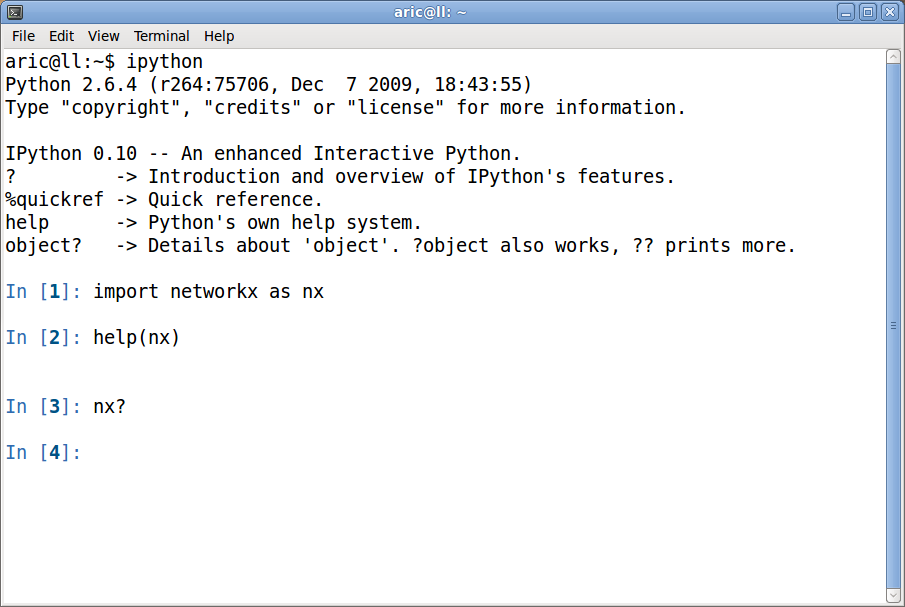
\includegraphics[width=4.0in]{nx-ipython}}
No GUI \footnotesize{http://www.cryptonomicon.com/beginning.html}
\end{frame}

\begin{frame}
\frametitle{Command line vs executing file}
You can type commands interactively or put them in a file and run them.
\centerline{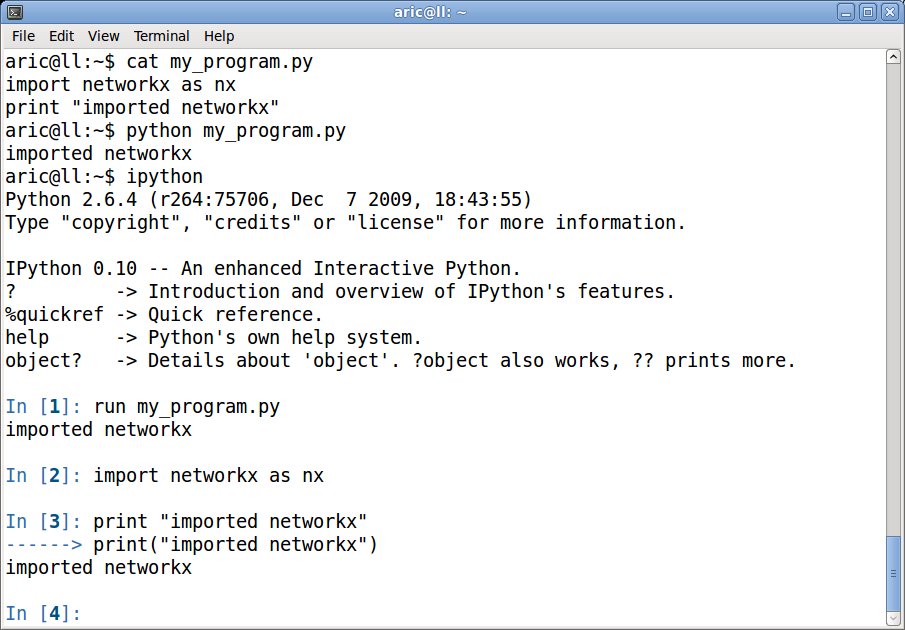
\includegraphics[width=4.0in]{ipython-import}}
\end{frame}

\begin{frame}
\frametitle{The > > > (doctests)}
\centerline{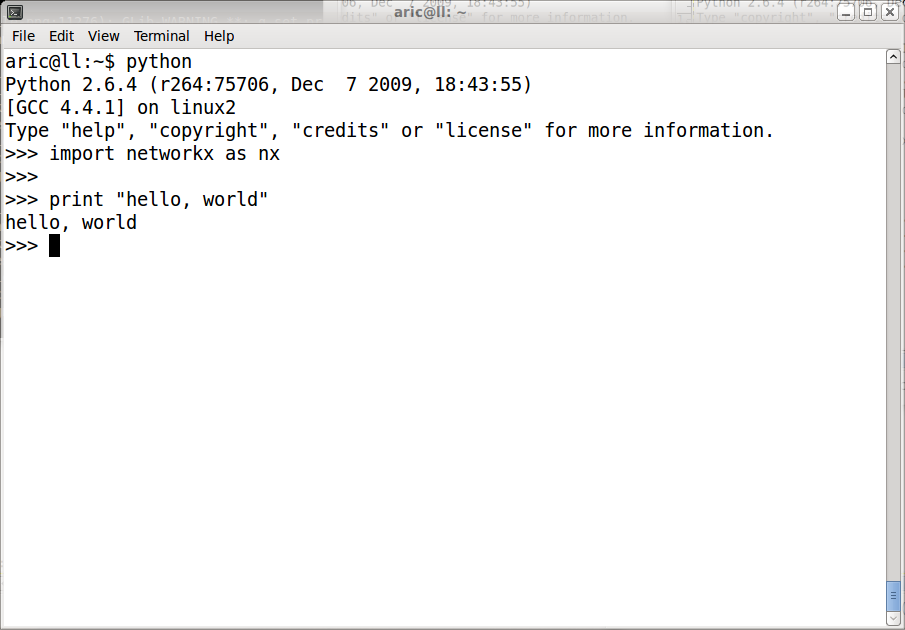
\includegraphics[width=4.0in]{python-hello}}
%\centerline{\includegraphics{python-hello-small}}

\end{frame}

\begin{frame}
\frametitle{Creating a graph}

The basic $Graph$ object is used to hold the network information.

Create an empty graph with no nodes and no edges:

\begin{block}{}
\lstinputlisting[firstline=1,lastline=4]{code/build_graph.py.doctest}
\end{block}

The graph G can be grown in several ways.

NetworkX includes many graph generator functions 
and facilities to read and write graphs in many formats.
\end{frame}

% FIXME interactive command line IPython, vs Python vs file

\begin{frame}[fragile]
\frametitle{Adding nodes}

\begin{block}{}
\lstinputlisting[firstline=5,lastline=17]{code/build_graph.py.doctest}
\end{block}

Nodes can be any hashable object such as strings,
numbers, files, functions, and more.

\end{frame}



\begin{frame}[fragile]

G can also be grown by adding edges.

\begin{block}{}
\lstinputlisting[firstline=18,lastline=35]{code/build_graph.py.doctest}

\end{block}

If the nodes do not already exist they are automatically added to the graph.

You can demolish the graph similarly with 
\begin{verbatim}
G.remove_node, G.remove_nodes_from, 
G.remove_edge, G.remove_edges_from.
\end{verbatim}

\end{frame}

% One can demolish the graph in a similar fashion; using 
% :meth:`Graph.remove_node`,
% :meth:`Graph.remove_nodes_from`, 
% :meth:`Graph.remove_edge`
% and 
% :meth:`Graph.remove_edges_from`, e.g.


\begin{frame}
\Large
\begin{itemize}

\item How do I find out the names of the methods like add\_edge?

\item How do I see what is in my graph?

\end{itemize}
\end{frame}

\begin{frame}
\frametitle{What's in NetworkX?}
\centerline{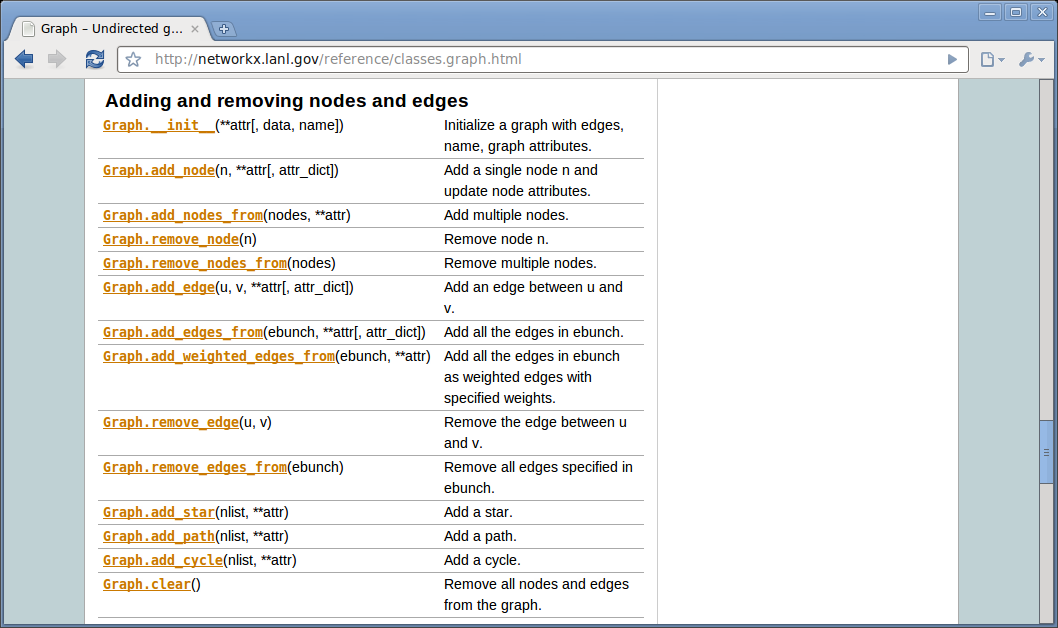
\includegraphics[width=1.0\columnwidth]{nx-doc-add}}
\end{frame}

\begin{frame}
\frametitle{What's in NetworkX?}
\centerline{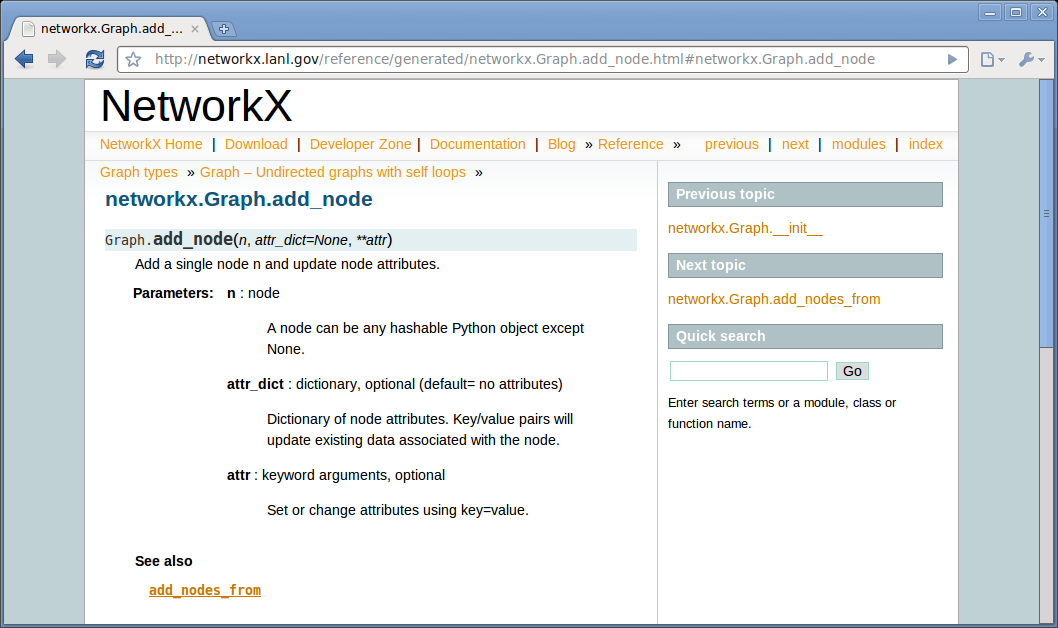
\includegraphics[width=1.0\columnwidth]{nx-doc-add-1}}
\end{frame}

\begin{frame}
\frametitle{What's in Networkx?}
\centerline{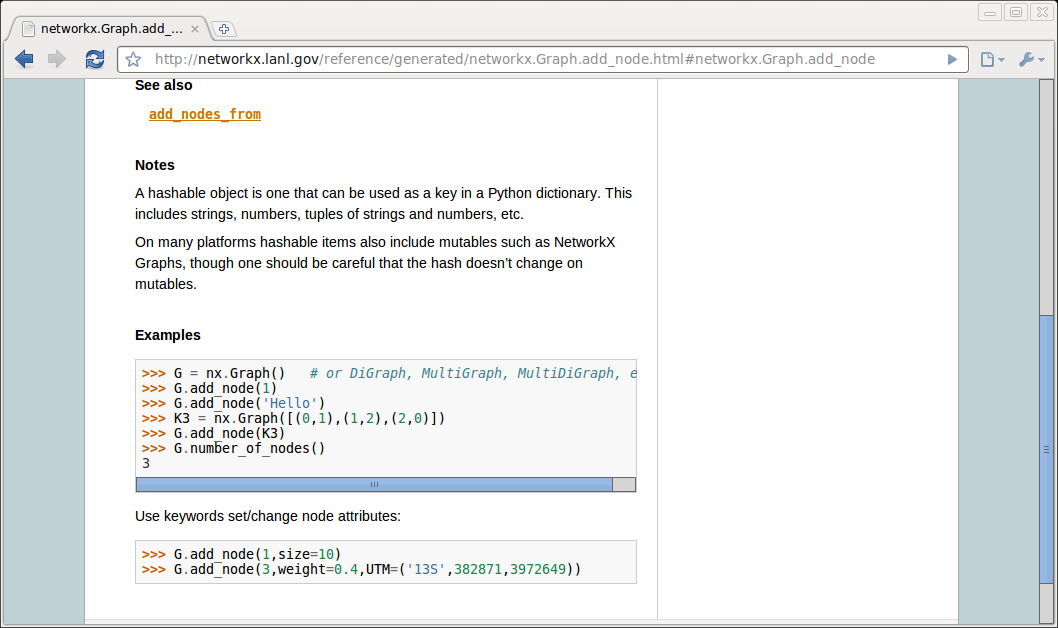
\includegraphics[width=1.0\columnwidth]{nx-doc-add-2}}
\end{frame}

\begin{frame}
\frametitle{What's in Networkx?}
\centerline{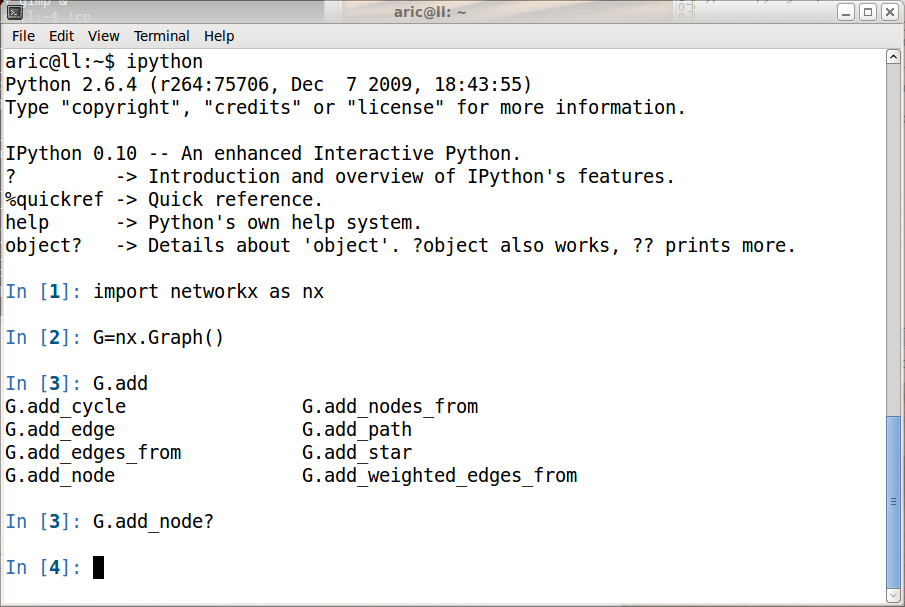
\includegraphics[width=4.0in]{nx-ipython-tab}}
\end{frame}

\begin{frame}
\frametitle{What's in Networkx?}
\centerline{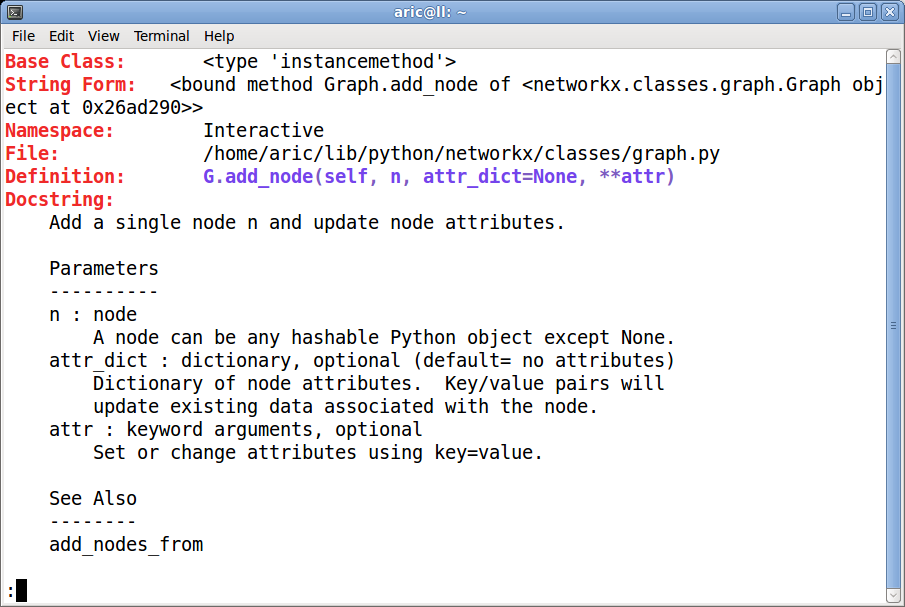
\includegraphics[width=4.0in]{nx-ipython-tab-add}}
\end{frame}


\begin{frame}
\frametitle{What's in Networkx?}
\centerline{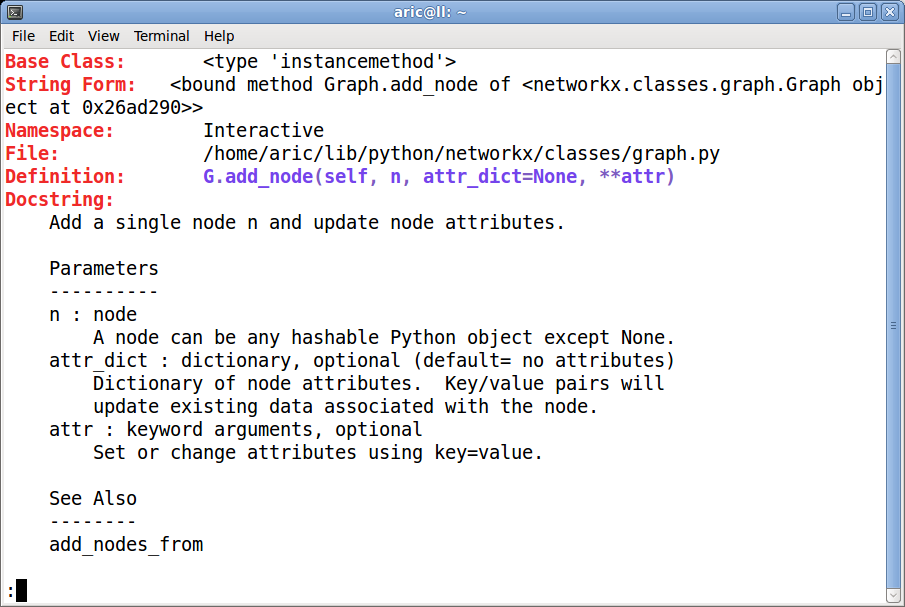
\includegraphics[width=4.0in]{nx-ipython-tab-add}}
Demo
\end{frame}


% show how to run file
% run 
% G.number_of_nodes()
% G.number_of_edges()
% G.nodes()
% G.edges()

\begin{frame}[fragile]
\frametitle{Adding attributes to graphs, nodes, and edges}

\begin{columns}
\begin{column}{0.3\textwidth}

(Almost) any Python object is allowed as graph, node, and edge data. 
\begin{itemize}
\item number
\item string
\item image
\item IP address
\item email address
\end{itemize}
\end{column}

\begin{column}{0.7\textwidth}
\centerline{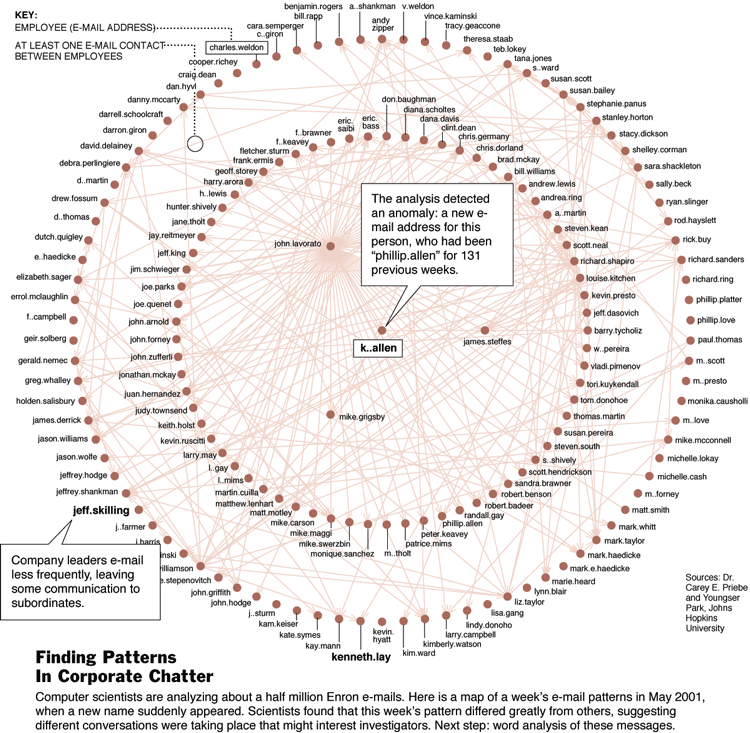
\includegraphics[width=1.0\columnwidth]{enron}}
\end{column}

\end{columns}

%Data assigned and stored in a Python dictionaries (default empty).
%(But what are dictionaries? more later...)

\end{frame}


\begin{frame}[fragile]
\frametitle{Graph attributes}
\lstinputlisting[firstline=1,lastline=12]{code/attributes.py.doctest}

\end{frame}



\begin{frame}[fragile]
\frametitle{Node attributes}
\lstinputlisting[firstline=13,lastline=25]{code/attributes.py.doctest}

\end{frame}

\begin{frame}[fragile]
\frametitle{Edge attributes}
\lstinputlisting[firstline=27,lastline=45]{code/attributes.py.doctest}

\end{frame}

\begin{frame}[fragile]
\frametitle{Weighted graph example}
\begin{columns}
\begin{column}{0.7\textwidth}
The special attribute 'weight'
should be numeric and holds values used by algorithms requiring weighted edges.

Use Dijkstra's algorithm to find the shortest path:

\end{column}

\begin{column}{0.3\textwidth}
\centerline{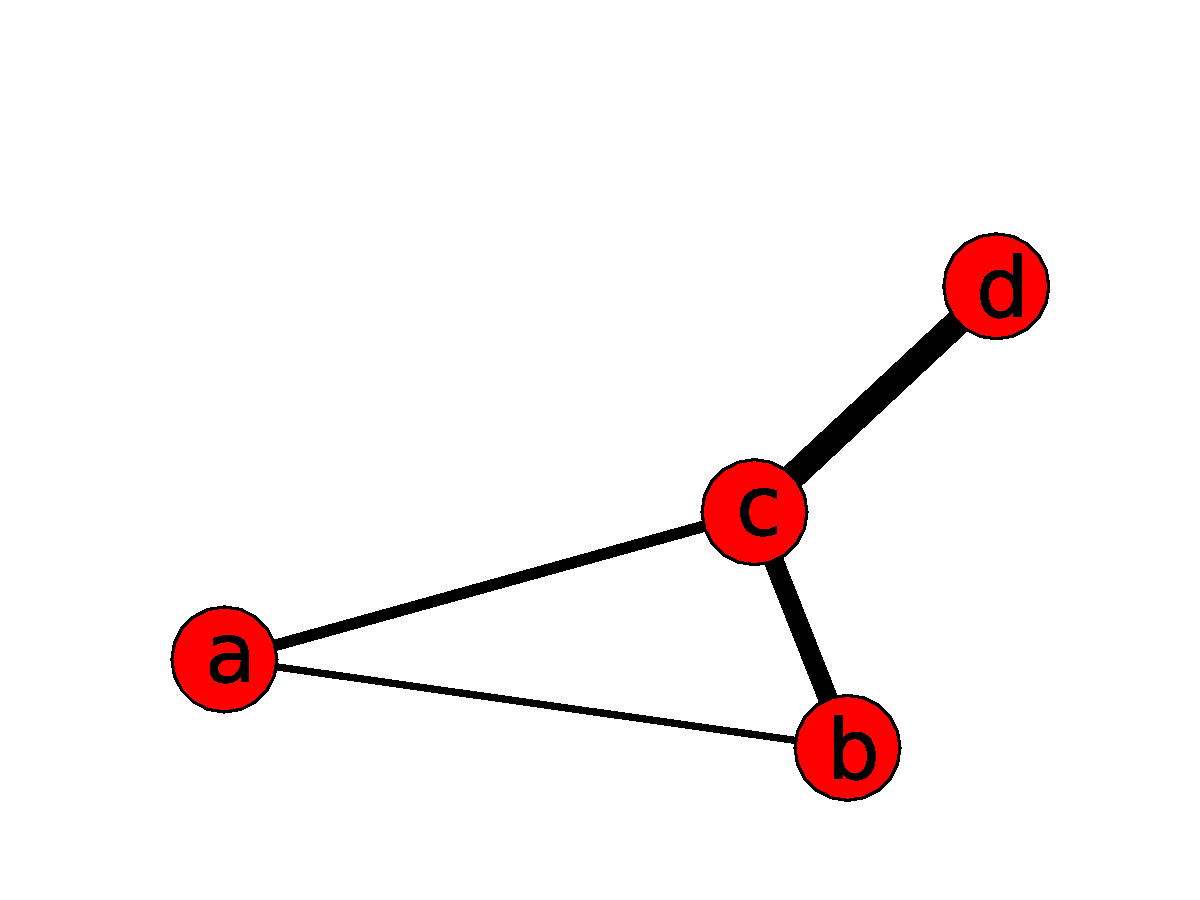
\includegraphics[width=1.4\columnwidth]{dijkstra}}
\end{column}
\end{columns}

\begin{block}{}
\lstinputlisting{code/dijkstra.py.doctest}
\end{block}

\end{frame}

\begin{frame}[fragile]
\frametitle{More ways to build graphs: operators and generators}

Applying classic graph operations

\begin{description}

\item[subgraph(G, nbunch)]      - induce subgraph of G on nodes in nbunch
\item[union(G1,G2)]             - graph union
\item[disjoint\_union(G1,G2)]    - graph union assuming all nodes are different
\item[cartesian\_product(G1,G2)] - return Cartesian product graph
\item[compose(G1,G2)]           - combine graphs identifying nodes common to both
\item[complement(G)]            - graph complement 
\item[create\_empty\_copy(G)]     - return an empty copy of the same graph class
\item[convert\_to\_undirected(G)] - return an undirected representation of G
\item[convert\_to\_directed(G)]   - return a directed representation of G
\end{description}

\end{frame}

\begin{frame}
\frametitle{Call a graph generator}

\lstinputlisting[firstline=2]{code/generators.py.doctest}
\end{frame}

% FIXME add examples
\begin{frame}
 Read a graph stored in a file using common graph formats. 
\begin{description}
\item [edge lists]
\item [adjacency lists]
\item [GML]
\item [GraphML]
\item [Pajek]
\item [LEDA]
\end{description}

\end{frame}


% FIXME switch to interactive and show example of paste
\begin{frame}[fragile]
\frametitle{Basic analysis of graphs}

\lstinputlisting[firstline=2]{code/analysis.py.doctest}

% For values of specific nodes, you can provide a single node or an nbunch 
% of nodes as argument.  If a single node is specified, then a single value 
% is returned.  If an nbunch is specified, then the function will 
% return a dictionary.
 
% >>> nx.degree(G,1)
% 2
% >>> G.degree(1)
% 2
% >>> G.degree([1,2])
% {1: 2, 2: 1}
% >>> sorted(G.degree([1,2]).values())
% [1, 2]
% >>> sorted(G.degree().values())
% [0, 1, 1, 2]

\end{frame}


% \begin{frame}[fragile]
% \frametitle{Inside NetworkX}

% It's ``Python all the way down''

% NetworkX uses a ``dictionary of dictionaries''

% Good for adjacency list representation (sparse graphs)

% \begin{itemize}
%   \item Node $n$ is a key in the $G.adj$ dictionary 
%   \item Data is a dictionary with neighbors as keys and data $1$
% \end{itemize}

% Representation of an undirected graph with the edges $A-B$, $B-C$
% \begin{block}{}
% \begin{verbatim}
% >>> G=nx.Graph()
% >>> G.add_edge('A','B')
% >>> G.add_edge('B','C')
% >>> print G.adj
% {'A': {'B': 1}, 
%  'B': {'A': 1, 'C': 1}, 
%  'C': {'B': 1}}
% \end{verbatim}
% \end{block}
% \end{frame}

% \begin{frame}[fragile]
% \frametitle{Dictionary of dictionaries}

% Guido van Rossum proposed a dictionary of lists 

% Allows the natural expressions (Eppstein)

% \begin{itemize}
%     \item ``{\tt n in G}'' to test if the graph $G$ contains node $n$ 
%     \item ``{\tt for n in G}'' to loop over all nodes
% \end{itemize}

% Advantages of ``dict of dict'' data structure
  
% \begin{itemize}
%   \item Find edges and remove edges with two dictionary look-ups 
%   \item Prefer to ``sets'' since data can be attached to edge
%     \begin{itemize}
%       \item $G[u][v]$ returns the edge object
%     \end{itemize}
% \end{itemize}

% \footnotesize

% \begin{itemize}
% \item
% Guido van Rossum.
% Python {P}atterns - {I}mplementing {G}raphs, 1998.
% \url{http://www.python.org/doc/essays/graphs/}

% \item
% David Eppstein.
% {PADS}, a library of {P}ython {A}lgorithms and {D}ata {S}tructures,
%   2008.
% \url{http://www.ics.uci.edu/\~eppstein/PADS/}
% \end{itemize}

% \end{frame}




\end{document}
